\documentclass[aspectratio=169]{beamer}
\usetheme{Madrid}
\usecolortheme{default}

% Packages
\usepackage{tikz}
\usepackage{algorithm}
\usepackage{algorithmic}
\usepackage{amsmath}
\usepackage{amssymb}
\usepackage{booktabs}
\usepackage{graphicx}

% TikZ libraries
\usetikzlibrary{shapes,arrows,positioning,calc,backgrounds,fit,decorations.pathreplacing}

% Custom colors
\definecolor{maincolor}{RGB}{0,102,204}
\definecolor{accentcolor}{RGB}{255,102,0}
\definecolor{lightgray}{RGB}{240,240,240}
\definecolor{successcolor}{RGB}{46,125,50}

% Title information
\title[MOEA/D]{MOEA/D: A Multiobjective Evolutionary Algorithm\\Based on Decomposition}
\subtitle{An Intuitive Guide from Basics to Implementation}
\author{Based on Zhang \& Li (2007)}
\date{\today}

\begin{document}

% =============================================================================
% TITLE AND INTRODUCTION
% =============================================================================
\begin{frame}{MOEA/D: The Idea of Decomposition}
\begin{center}

\vspace{0.6em}
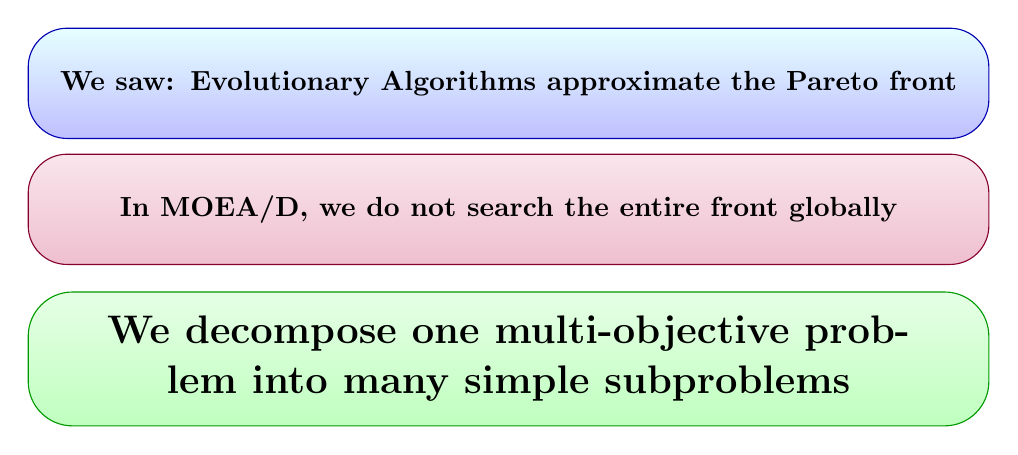
\begin{tikzpicture}

% -------- Top context box --------
\node[
draw=blue!70!black,
rounded corners=14pt,
top color=cyan!10,
bottom color=blue!25,
minimum width=12.2cm,
minimum height=1.4cm,
text width=11.8cm,
align=center,
font=\normalsize\bfseries
] at (0,2.1)
{We saw: Evolutionary Algorithms approximate the Pareto front};

% -------- Middle statement box --------
\node[
draw=purple!70!black,
rounded corners=14pt,
top color=purple!10,
bottom color=purple!25,
minimum width=12.2cm,
minimum height=1.4cm,
text width=11.8cm,
align=center,
font=\normalsize\bfseries
] at (0,0.5)
{In MOEA/D, we do not search the entire front globally};

% -------- Key idea box --------
\node[
draw=green!60!black,
rounded corners=16pt,
top color=green!10,
bottom color=green!25,
minimum width=12.2cm,
minimum height=1.7cm,
text width=11.8cm,
align=center,
font=\Large\bfseries
] at (0,-1.4)
{We decompose one multi-objective problem into many simple subproblems};

\end{tikzpicture}

\end{center}
\end{frame}



\begin{frame}{The Idea of Decomposition}
\begin{center}

\vspace{0.7em}

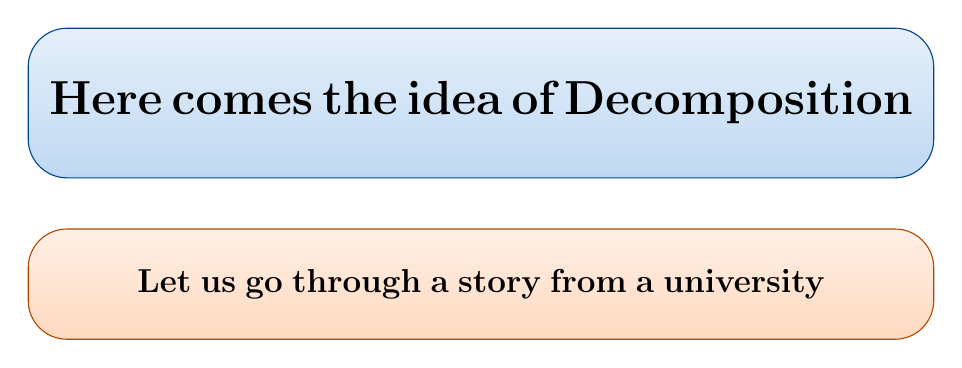
\begin{tikzpicture}

% -------- Top box (MAIN, bigger) --------
\node[
draw=maincolor!70!black,
rounded corners=14pt,
top color=maincolor!10,
bottom color=maincolor!25,
minimum width=11.5cm,
minimum height=1.9cm,
text width=11.0cm,
align=center
] at (0,1.4)
{{\LARGE\bfseries Here comes the idea of Decomposition}};

% -------- Bottom box (smaller) --------
\node[
draw=accentcolor!70!black,
rounded corners=14pt,
top color=accentcolor!10,
bottom color=accentcolor!25,
minimum width=11.5cm,
minimum height=1.4cm,
text width=11.0cm,
align=center
] at (0,-0.9)
{{\large\bfseries Let us go through a story from a university}};

\end{tikzpicture}

\end{center}
\end{frame}
% ------ Slide 1: Scene Setting ------
\begin{frame}{It's That Time of Year...}
\begin{center}


\begin{tikzpicture}

% -------- Main title card (forced single line) --------
\node[
draw=blue!70!black,
rounded corners=18pt,
top color=cyan!10,
bottom color=blue!25,
minimum width=11.2cm,
minimum height=2.6cm,
align=center
] at (0,0.4)
{{\LARGE\bfseries University Scholarship Selection Season}};

% -------- Role box --------
\node[
draw=green!70!black,
rounded corners=14pt,
top color=green!10,
bottom color=green!45,
minimum width=9.0cm,
minimum height=1.6cm,
text width=8.5cm,
align=center
] at (0,-2.0)
{{\large You are on the \textbf{Selection Committee}\\
Your task: choose the most deserving candidates.}};

\end{tikzpicture}

\end{center}
\end{frame}


% ------ Slide 2: The Stack ------
\begin{frame}{The Stack on Your Desk}
\begin{center}
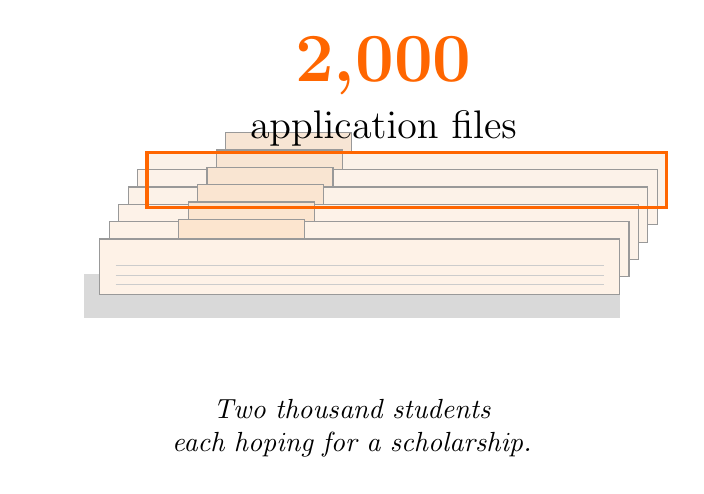
\begin{tikzpicture}

% Shadow
\fill[black!15] (-3.4,-0.3) rectangle (3.4,0.25);

% File stack
\foreach \i in {5,4,3,2,1,0} {

  % Folder body
  \filldraw[
    draw=black!40,
    fill=brown!\the\numexpr 20+\i*8\relax!orange!10
  ]
  (\i*0.12-3.2, \i*0.22)
  rectangle ++(6.6,0.7);

  % Folder tab
  \filldraw[
    draw=black!40,
    fill=brown!\the\numexpr 25+\i*8\relax!orange!20
  ]
  (\i*0.12-2.2, \i*0.22+0.7)
  rectangle ++(1.6,0.25);

  % Paper lines inside (top 2 folders only for realism)
  \ifnum\i<2
    \foreach \y in {0.12,0.24,0.36} {
      \draw[black!20] (\i*0.12-3.0, \i*0.22+\y) -- ++(6.2,0);
    }
  \fi
}

% Highlight top file border
\draw[accentcolor, line width=1.2pt]
(5*0.12-3.2,5*0.22) rectangle ++(6.6,0.7);

% Big number (moved higher)
\node[
  font=\fontsize{42}{42}\bfseries,
  text=accentcolor
] at (0.4,2.9) {2,000};

% Subtitle (now above the stack)
\node[
  font=\Large,
  text=black
] at (0.4,2.1) {application files};

% Caption
\node[
  font=\normalsize\itshape,
  text width=8cm,
  align=center
] at (0, -1.7)
{Two thousand students\\
each hoping for a scholarship.};

\end{tikzpicture}
\end{center}
\end{frame}

% ------ Slide 3: Meet the Applicants ------
\begin{frame}{You Open the First Few Files...}
\begin{center}
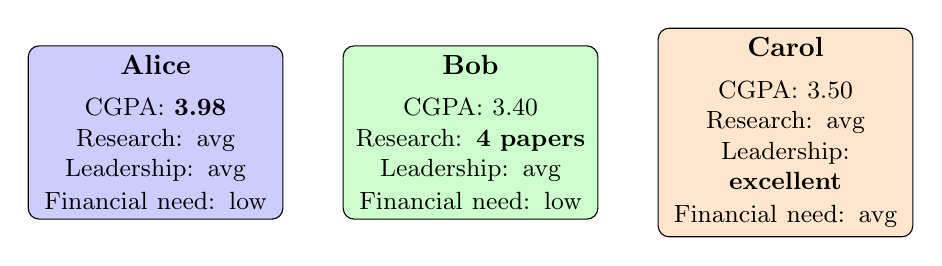
\begin{tikzpicture}[
  card/.style={draw, rounded corners, fill=#1, minimum width=3.2cm,
               minimum height=2.2cm, text width=3cm, align=center}]

  \node[card=blue!20]   at (0,   0) {\textbf{Alice}\\[0.4em]
                                      \small CGPA: \textbf{3.98}\\
                                      Research: avg\\
                                      Leadership: avg\\
                                      Financial need: low};

  \node[card=green!20]  at (4,   0) {\textbf{Bob}\\[0.4em]
                                      \small CGPA: 3.40\\
                                      Research: \textbf{4 papers}\\
                                      Leadership: avg\\
                                      Financial need: low};

  \node[card=orange!20] at (8,   0) {\textbf{Carol}\\[0.4em]
                                      \small CGPA: 3.50\\
                                      Research: avg\\
                                      Leadership: \textbf{excellent}\\
                                      Financial need: avg};
\end{tikzpicture}
\end{center}
\end{frame}


% ------ Slide 4: And More... ------
\begin{frame}{...And More Files}
\begin{center}

\begin{tikzpicture}[
  card/.style={draw, rounded corners, fill=#1, minimum width=3.2cm,
               minimum height=2.2cm, text width=3cm, align=center}]

  \node[card=red!20]    at (0,   0) {\textbf{Dave}\\[0.4em]
                                      \small CGPA: 3.10\\
                                      Research: low\\
                                      Leadership: avg\\
                                      Financial need: \textbf{very high}};

  \node[card=purple!15] at (4,   0) {\textbf{Eva}\\[0.4em]
                                      \small CGPA: 3.70\\
                                      Research: \textbf{3 papers}\\
                                      Leadership: \textbf{good}\\
                                      Financial need: avg};

  \node[font=\normalsize\itshape, text width=5cm, align=center] at (8, 0)
       {$\cdots$ and 1,995 more just like these.};

\end{tikzpicture}
\end{center}
\end{frame}


% ------ Slide 5: Naive Question ------
\begin{frame}{The Obvious Question}
\begin{center}
\vspace{1em}
{\LARGE \textbf{``JUST RANK THEM!!!''}}

\vspace{2em}

\begin{tikzpicture}
  \node[draw, rounded corners, fill=gray!10, minimum width=8cm,
        minimum height=1.5cm, text width=7.8cm, align=center, font=\large] at (0,0)
       {Assign a score to each applicant.\\
        Sort from best to worst. Pick the top ones.};
\end{tikzpicture}

\vspace{2em}
{\large Sounds simple, right?}
\end{center}
\end{frame}


% ------ Slide 6: But wait... ------
\begin{frame}{But Wait --- What's the Score?}
\begin{center}
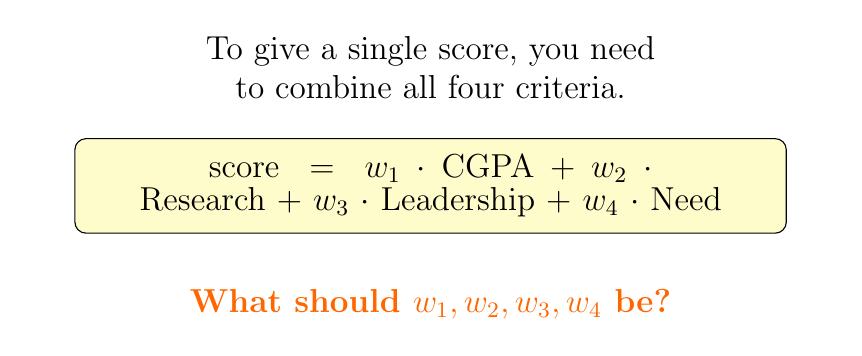
\begin{tikzpicture}
  \node[font=\large, text width=10cm, align=center] at (0, 1.5)
       {To give a single score, you need to combine all four criteria.};

  \node[draw, rounded corners, fill=yellow!20, minimum width=9cm,
        minimum height=1.2cm, text width=8.8cm, align=center] at (0, 0)
       {\large $\text{score} = w_1 \cdot \text{CGPA} + w_2 \cdot \text{Research} + w_3 \cdot \text{Leadership} + w_4 \cdot \text{Need}$};

  \node[font=\large\bfseries, text=accentcolor] at (0, -1.5)
       {What should $w_1, w_2, w_3, w_4$ be?};
\end{tikzpicture}
\end{center}
\end{frame}


% ------ Slide 7: The Weight Problem ------
\begin{frame}{Nobody Agrees on the Weights}
\begin{center}
\begin{tikzpicture}[
bubble/.style={
draw=black!50,
rounded corners=10pt,
fill=#1,
minimum width=3.2cm,
minimum height=2.1cm,
text width=2.7cm,
align=center,
font=\small,
drop shadow
},
tail/.style={draw=black!50, fill=#1}
]

% -------- Prof A --------
\node[bubble=blue!15] (A) at (0,2)
{Prof.\ A:\\[0.2em]
\textit{``CGPA is everything!''}};
\draw[tail=blue!15] (-0.6,1.2) -- (-0.3,1.5) -- (-0.1,1.1) -- cycle;

% -------- Prof B --------
\node[bubble=green!15] (B) at (4.5,2)
{Prof.\ B:\\[0.2em]
\textit{``Research matters most.''}};
\draw[tail=green!15] (3.9,1.2) -- (4.2,1.5) -- (4.4,1.1) -- cycle;

% -------- Prof C --------
\node[bubble=orange!15] (C) at (0,-0.8)
{Prof.\ C:\\[0.2em]
\textit{``We need leaders!''}};
\draw[tail=orange!15] (-0.6,-1.6) -- (-0.3,-1.3) -- (-0.1,-1.7) -- cycle;

% -------- Prof D --------
\node[bubble=red!15] (D) at (4.5,-0.8)
{Prof.\ D:\\[0.2em]
\textit{``Financial need is priority.''}};
\draw[tail=red!15] (3.9,-1.6) -- (4.2,-1.3) -- (4.4,-1.7) -- cycle;

% -------- Right-side summary --------
\node[
font=\large\itshape,
text width=5.2cm,
align=center
] at (9.2,0.6)
{Every committee member has a \textbf{different} notion of ``best''.};

\end{tikzpicture}
\end{center}
\end{frame}


% ------ Slide 8: Try Anyway --- Compare Alice vs Bob ------
\begin{frame}{Okay, Let's Try. Who's Better: Alice or Bob?}
\begin{center}
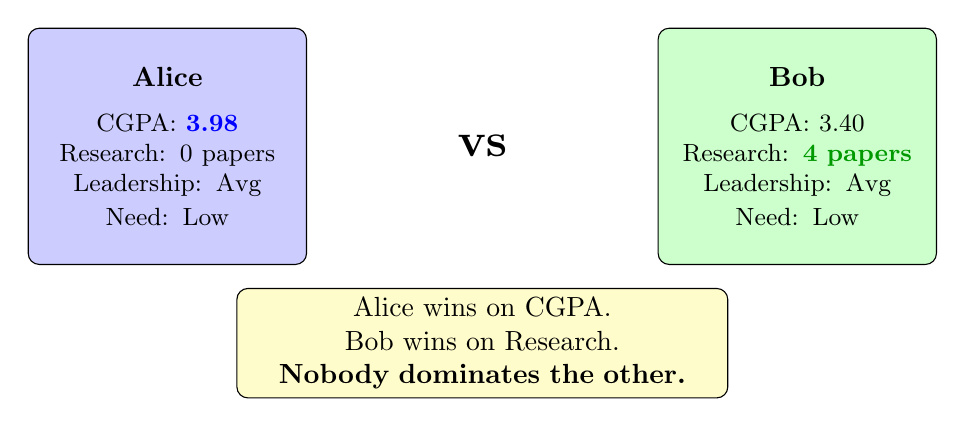
\begin{tikzpicture}
  \node[draw, rounded corners, fill=blue!20, minimum width=3.5cm, minimum height=3cm,
        text width=3.3cm, align=center] (alice) at (0, 0)
       {\textbf{Alice}\\[0.5em]
        \small CGPA: \textcolor{blue}{\textbf{3.98}}\\
        Research: 0 papers\\
        Leadership: Avg\\
        Need: Low};

  \node[font=\LARGE\bfseries] at (4, 0) {vs};

  \node[draw, rounded corners, fill=green!20, minimum width=3.5cm, minimum height=3cm,
        text width=3.3cm, align=center] (bob) at (8, 0)
       {\textbf{Bob}\\[0.5em]
        \small CGPA: 3.40\\
        Research: \textcolor{green!60!black}{\textbf{4 papers}}\\
        Leadership: Avg\\
        Need: Low};

  \node[draw, rounded corners, fill=yellow!20, text width=6cm, align=center,
        font=\normalsize] at (4, -2.5)
       {Alice wins on CGPA.\\
        Bob wins on Research.\\
        \textbf{Nobody dominates the other.}};
\end{tikzpicture}
\end{center}
\end{frame}


% ------ Slide 9: Now scale it up ------
\begin{frame}{Now Do That for 2,000 Applicants}
\begin{center}
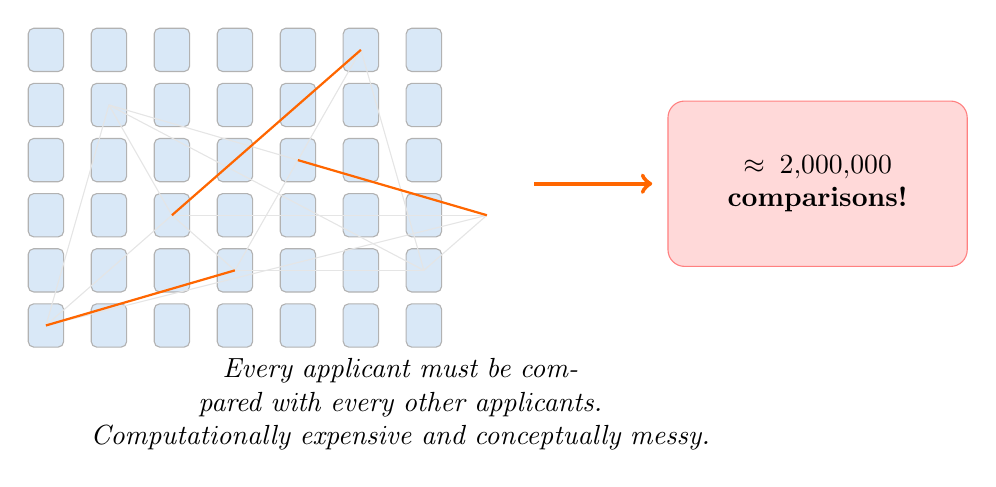
\begin{tikzpicture}[scale=1]

% ---- Mini applicant cards (grid) ----
\foreach \x in {0,0.8,...,5.6} {
  \foreach \y in {0,0.7,...,3.5} {
    \node[
      draw=black!30,
      fill=maincolor!15,
      rounded corners=2pt,
      minimum width=0.45cm,
      minimum height=0.55cm
    ] at (\x,\y) {};
  }
}

% ---- Light comparison mesh (background) ----
\foreach \a/\b in {0/0,1.6/1.4,3.2/2.1,4.8/0.7} {
  \foreach \c/\d in {0.8/2.8,2.4/0.7,4/3.5,5.6/1.4} {
    \draw[gray!20] (\a,\b) -- (\c,\d);
  }
}

% ---- Highlight a few comparisons ----
\draw[accentcolor, thick] (0,0) -- (2.4,0.7);
\draw[accentcolor, thick] (1.6,1.4) -- (4,3.5);
\draw[accentcolor, thick] (3.2,2.1) -- (5.6,1.4);

% ---- Arrow to explosion box ----
\draw[->, ultra thick, accentcolor] (6.2, 1.8) -- (7.7, 1.8);

% ---- Result box ----
\node[
draw=red!50,
rounded corners=6pt,
fill=red!15,
minimum width=3.8cm,
minimum height=2.1cm,
text width=3.4cm,
align=center,
font=\bfseries
] at (9.8, 1.8)
{$\approx 2{,}000{,}000$\\comparisons!};

% ---- Caption ----
\node[
font=\normalsize\itshape,
text width=9cm,
align=center
] at (4.5, -1.0)
{Every applicant must be compared with every other applicants.\\
Computationally expensive \textit{and} conceptually messy.};

\end{tikzpicture}
\end{center}
\end{frame}

% ------ Slide 10: Diversity Problem ------
\begin{frame}{And Even If You Do It...}
\begin{center}
\textbf{\large Final Top 10 Selected:}

\vspace{0.6em}
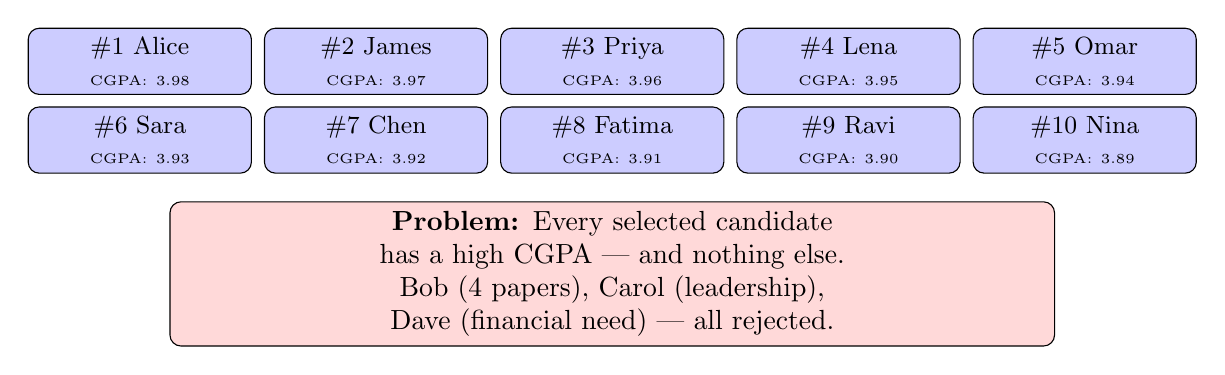
\begin{tikzpicture}
  % Row 1
  \node[draw, fill=blue!20, rounded corners, minimum width=2.8cm, font=\small,
        minimum height=0.65cm, text width=2.6cm, align=center] at (0*3.0, 1.2)
        {\#1 Alice\\\tiny CGPA: 3.98};
  \node[draw, fill=blue!20, rounded corners, minimum width=2.8cm, font=\small,
        minimum height=0.65cm, text width=2.6cm, align=center] at (1*3.0, 1.2)
        {\#2 James\\\tiny CGPA: 3.97};
  \node[draw, fill=blue!20, rounded corners, minimum width=2.8cm, font=\small,
        minimum height=0.65cm, text width=2.6cm, align=center] at (2*3.0, 1.2)
        {\#3 Priya\\\tiny CGPA: 3.96};
  \node[draw, fill=blue!20, rounded corners, minimum width=2.8cm, font=\small,
        minimum height=0.65cm, text width=2.6cm, align=center] at (3*3.0, 1.2)
        {\#4 Lena\\\tiny CGPA: 3.95};
  \node[draw, fill=blue!20, rounded corners, minimum width=2.8cm, font=\small,
        minimum height=0.65cm, text width=2.6cm, align=center] at (4*3.0, 1.2)
        {\#5 Omar\\\tiny CGPA: 3.94};
  % Row 2
  \node[draw, fill=blue!20, rounded corners, minimum width=2.8cm, font=\small,
        minimum height=0.65cm, text width=2.6cm, align=center] at (0*3.0, 0.2)
        {\#6 Sara\\\tiny CGPA: 3.93};
  \node[draw, fill=blue!20, rounded corners, minimum width=2.8cm, font=\small,
        minimum height=0.65cm, text width=2.6cm, align=center] at (1*3.0, 0.2)
        {\#7 Chen\\\tiny CGPA: 3.92};
  \node[draw, fill=blue!20, rounded corners, minimum width=2.8cm, font=\small,
        minimum height=0.65cm, text width=2.6cm, align=center] at (2*3.0, 0.2)
        {\#8 Fatima\\\tiny CGPA: 3.91};
  \node[draw, fill=blue!20, rounded corners, minimum width=2.8cm, font=\small,
        minimum height=0.65cm, text width=2.6cm, align=center] at (3*3.0, 0.2)
        {\#9 Ravi\\\tiny CGPA: 3.90};
  \node[draw, fill=blue!20, rounded corners, minimum width=2.8cm, font=\small,
        minimum height=0.65cm, text width=2.6cm, align=center] at (4*3.0, 0.2)
        {\#10 Nina\\\tiny CGPA: 3.89};

  \node[draw, rounded corners, fill=red!15, text width=11cm, align=center,
        font=\normalsize, minimum height=1.2cm] at (6.0, -1.5)
       {\textbf{Problem:} Every selected candidate has a high CGPA --- and nothing else.\\
        Bob (4 papers), Carol (leadership), Dave (financial need) --- all rejected.};
\end{tikzpicture}
\end{center}
\end{frame}


% ------ Slide 11: The Real Issue ------
\begin{frame}{The Real Issue}
\begin{center}
\vspace{0.5em}
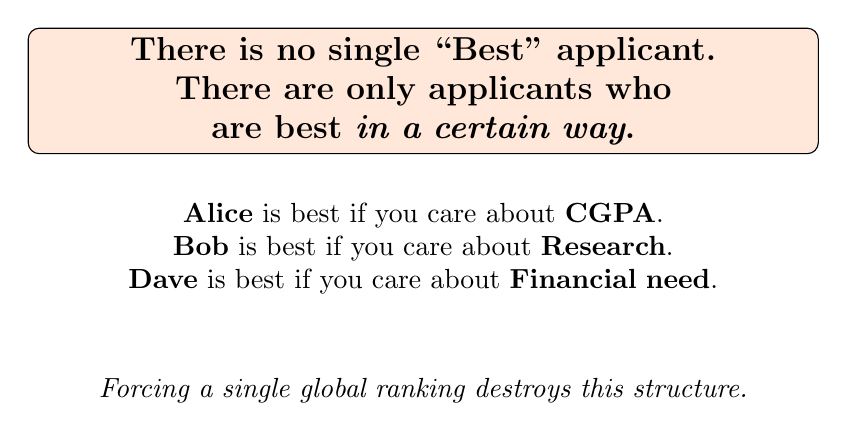
\begin{tikzpicture}
  \node[draw, rounded corners, fill=accentcolor!15, minimum width=10cm,
        minimum height=1.5cm, text width=9.8cm, align=center, font=\large\bfseries] at (0, 1.5)
       {There is no single ``Best'' applicant.\\
        There are only applicants who are best \textit{in a certain way}.};

  \node[font=\normalsize, text width=9cm, align=center] at (0, -0.5)
       {\textbf{Alice} is best if you care about \textbf{CGPA}.\\
        \textbf{Bob} is best if you care about \textbf{Research}.\\
        \textbf{Dave} is best if you care about \textbf{Financial need}.};

  \node[font=\normalsize\itshape, text width=9cm, align=center] at (0, -2.3)
       {Forcing a single global ranking destroys this structure.};
\end{tikzpicture}
\end{center}
\end{frame}


% ------ Slide 12: A Better Idea Emerges ------
\begin{frame}{A Better Idea Starts to Form...}
\begin{center}

{\large What if we \textbf{stopped} trying to build one global ranking...}

\vspace{1.4em}

\begin{tikzpicture}

% -------- Top box: global ranking --------
\node[
draw=red!60!black,
line width=1pt,
rounded corners=8pt,
top color=red!10,
bottom color=red!25,
minimum width=9cm,
minimum height=1.3cm,
text width=8.4cm,
align=center,
font=\bfseries,
drop shadow
] (global) at (0,0)
{One hard global ranking\\
(expensive, unfair, not diverse)};

% Arrow
\draw[->, ultra thick, accentcolor] (0,-0.85) -- (0,-1.75);

% -------- Bottom box: decomposition idea --------
\node[
draw=successcolor!60!black,
line width=1pt,
rounded corners=8pt,
top color=successcolor!15,
bottom color=successcolor!30,
minimum width=9cm,
minimum height=1.3cm,
text width=8.4cm,
align=center,
font=\bfseries,
drop shadow
] (decomp) at (0,-2.6)
{Several focused sub-selections\\
(one per preference type)};

% Caption
\node[
font=\normalsize\itshape,
text width=8.5cm,
align=center
] at (0,-4.0)
{Each sub-problem is simple. Together, they cover everything.};

\end{tikzpicture}

\end{center}
\end{frame}


% ------ Slide 13: One Pattern Emerges ------



% ------ Slide 14: The Two Questions ------
\begin{frame}{Two Questions That Change Everything}
\begin{center}

\begin{tikzpicture}

% -------- Question 1 --------
\node[
draw=maincolor!70!black,
line width=1pt,
rounded corners=10pt,
top color=maincolor!10,
bottom color=maincolor!25,
minimum width=12cm,
minimum height=1.5cm,
align=center,
font=\large\bfseries,
drop shadow
] at (0,1.4)
{What if we stop building one global ranking?};

% -------- Question 2 --------
\node[
draw=accentcolor!70!black,
line width=1pt,
rounded corners=10pt,
top color=accentcolor!10,
bottom color=accentcolor!25,
minimum width=12cm,
minimum height=1.5cm,
align=center,
font=\large\bfseries,
drop shadow
] at (0,-0.6)
{What if we evaluate under different preferences instead?};

% -------- Caption --------
\node[
font=\normalsize\itshape,
text width=9cm,
align=center
] at (0,-2.8)
{These two questions lead us directly to the core idea behind \textbf{MOEA/D}.};

\end{tikzpicture}

\end{center}
\end{frame}



% =============================================================================
% STEP 1 — Preference-based Selection (continue scholarship story)
% =============================================================================



\begin{frame}{And Together, They Cover Everything}
\begin{center}
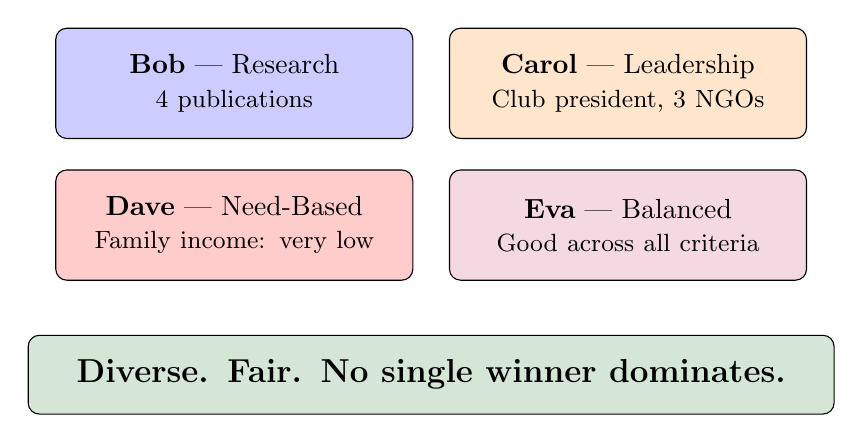
\begin{tikzpicture}[
  win/.style={draw, rounded corners, fill=#1, minimum width=4.5cm,
              minimum height=1.4cm, text width=4.3cm, align=center}]

  \node[win=blue!20]   at (0,   1.5) {\textbf{Bob} — Research\\{\small 4 publications}};
  \node[win=orange!20] at (5,   1.5) {\textbf{Carol} — Leadership\\{\small Club president, 3 NGOs}};
  \node[win=red!20]    at (0,  -0.3) {\textbf{Dave} — Need-Based\\{\small Family income: very low}};
  \node[win=purple!15] at (5,  -0.3) {\textbf{Eva} — Balanced\\{\small Good across all criteria}};

  \node[draw, rounded corners, fill=successcolor!20, text width=10cm, align=center,
        minimum height=1.0cm, font=\large\bfseries] at (2.5, -2.2)
       {Diverse. Fair. No single winner dominates.};
\end{tikzpicture}
\end{center}
\end{frame}


% =============================================================================
% STEP 2 — Insight Slide
% =============================================================================

\begin{frame}{The Key Insight}
\begin{center}
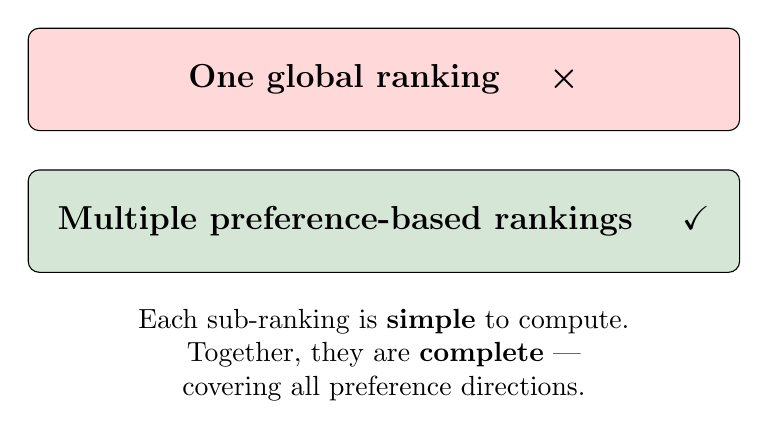
\begin{tikzpicture}
  \node[draw, rounded corners, fill=red!15, minimum width=9cm, minimum height=1.3cm,
        text width=8.8cm, align=center, font=\large\bfseries] at (0, 2)
       {One global ranking \quad $\boldsymbol{\times}$};

  \node[draw, rounded corners, fill=successcolor!20, minimum width=9cm, minimum height=1.3cm,
        text width=8.8cm, align=center, font=\large\bfseries] at (0, 0.2)
       {Multiple preference-based rankings \quad $\boldsymbol{\checkmark}$};

  \node[font=\normalsize, text width=8cm, align=center] at (0, -1.5)
       {Each sub-ranking is \textbf{simple} to compute.\\
        Together, they are \textbf{complete} — covering all preference directions.};
\end{tikzpicture}
\end{center}
\end{frame}


% =============================================================================
% STEP 3 — Map to Optimization + Introduce "Decomposition"
% =============================================================================




\begin{frame}{This Is Called: \textbf{Decomposition}}
\begin{center}

\vspace{0.4em}
{\LARGE Instead of one hard problem,}

\vspace{0.6em}
{\LARGE solve many simple ones.}

\vspace{1.2em}

\begin{tikzpicture}

% ---- Main Decomposition Box ----
\node[
draw=accentcolor!70!black,
line width=1pt,
rounded corners=10pt,
top color=accentcolor!10,
bottom color=accentcolor!25,
minimum width=11cm,
minimum height=1.5cm,
align=center,
font=\Large\bfseries,
drop shadow
] at (0,0)
{$\longrightarrow$ \quad Decomposition \quad $\longleftarrow$};

% ---- Definition Box ----
\node[
draw=maincolor!70!black,
line width=1pt,
rounded corners=8pt,
top color=maincolor!10,
bottom color=maincolor!20,
minimum width=11cm,
minimum height=1.2cm,
align=center,
font=\normalsize,
drop shadow
] at (0,-1.8)
{Breaking a multiobjective optimization problem\\
into multiple scalar subproblems, each with a different preference.};

\end{tikzpicture}

\vspace{1.1em}

{\normalsize One multiobjective problem \quad $\Rightarrow$ \quad many scalar subproblems}

\end{center}
\end{frame}


% =============================================================================
% STEP 4 — Visual Decomposition
% =============================================================================

\begin{frame}{Visualizing Decomposition}
\begin{center}
\begin{tikzpicture}[scale=0.95]

% ---- Hard problem box ----
\node[
draw=red!70!black,
line width=1pt,
rounded corners=8pt,
top color=red!10,
bottom color=red!25,
minimum width=4.8cm,
minimum height=1.6cm,
align=center,
font=\bfseries\large,
drop shadow
] (hard) at (0,2.5)
{One Hard\\Multiobjective Problem};

% ---- Arrow down ----
\draw[->, ultra thick, maincolor] (0,1.65) -- (0,0.9);
\node[font=\bfseries, text=maincolor] at (2.0,1.25) {Decompose};

% ---- Subproblem circles ----
\foreach \x/\g/\lbl in {
-4.6/g_1/Research focused,
-2.3/g_2/Leadership focused,
0/g_3/Balanced,
2.3/g_4/Need focused,
4.6/g_5/Academic focused}
{
\node[
draw=successcolor!70!black,
line width=0.9pt,
circle,
top color=successcolor!10,
bottom color=successcolor!30,
minimum size=1.25cm,
font=\bfseries,
drop shadow
] (\g) at (\x,-0.2) {$\g$};

\node[
font=\small,
text width=2.4cm,
align=center
] at (\x,-1.4) {\lbl};

\draw[->, thick, accentcolor] (0,0.9) -- (\g);
}

% ---- Bottom explanation box ----
\node[
draw=gray!60!black,
rounded corners=8pt,
top color=gray!5,
bottom color=gray!15,
minimum width=10.8cm,
minimum height=0.95cm,
align=center,
font=\normalsize,
drop shadow
] at (0,-2.6)
{Each $g_i$ is a \textbf{scalar} optimization problem — easy to solve individually.};

\end{tikzpicture}
\end{center}
\end{frame}


% =============================================================================
% PHONE STORY — Bridge from scholarship to objective space
% =============================================================================

\begin{frame}{A Second Story: Buying a Phone}
\begin{center}
\begin{tikzpicture}

% ---- Main card ----
\node[
draw=maincolor!70!black,
line width=1pt,
rounded corners=10pt,
top color=maincolor!10,
bottom color=maincolor!25,
minimum width=11cm,
minimum height=2.6cm,
align=center,
font=\Large\bfseries,
drop shadow
] at (0,0.2)
{You want to buy a new smartphone.};

% ---- Criteria text (manual line control, no awkward wrapping) ----
\node[
font=\normalsize,
align=center
] at (0,-2.0)
{You care about two things:\\[0.5em]
\textbf{1. Price} --- as low as possible \hspace{1.2cm}
\textbf{2. Camera Quality} --- as high as possible.};

\end{tikzpicture}
\end{center}
\end{frame}


\begin{frame}{You Walk Into the Store...}
\begin{center}
\begin{tikzpicture}[
phone/.style={
draw=#1!80!black,
line width=0.9pt,
rounded corners=10pt,
top color=#1!10,
bottom color=#1!25,
minimum width=3.4cm,
minimum height=3.1cm,
align=center,
font=\small,
drop shadow
}
]

% -------- Phone A --------
\node[phone=blue] at (0,0)
{\textbf{\large Phone A}\\[0.4em]
\textcolor{blue!70!black}{\textbf{\$200}}\\[0.3em]
Camera:\\
{\large\textbf{2/5}}\\[0.2em]
\tiny Budget pick};

% -------- Phone B --------
\node[phone=green!70!black] at (4.2,0)
{\textbf{\large Phone B}\\[0.4em]
\textbf{\$450}\\[0.3em]
Camera:\\
{\large\textbf{4/5}}\\[0.2em]
\tiny Mid-range};

% -------- Phone C --------
\node[phone=orange!80!black] at (8.4,0)
{\textbf{\large Phone C}\\[0.4em]
\textcolor{red!70!black}{\textbf{\$1{,}100}}\\[0.3em]
Camera:\\
{\large\textbf{5/5}}\\[0.2em]
\tiny Flagship};

% -------- Phone D --------
\node[phone=purple!70!black] at (12.6,0)
{\textbf{\large Phone D}\\[0.4em]
\textbf{\$500}\\[0.3em]
Camera:\\
{\large\textbf{2/5}}\\[0.2em]
\tiny Overpriced?};

\end{tikzpicture}
\end{center}
\end{frame}


\begin{frame}{Which One Is ``Best''?}
\begin{center}
\begin{tikzpicture}

% ---- Top statement ----
\node[
font=\large,
align=center
] at (0,2.1)
{It depends entirely on your \textbf{preference}.};

% ---- Budget winner ----
\node[
draw=blue!70!black,
line width=1pt,
rounded corners=10pt,
top color=blue!10,
bottom color=blue!25,
minimum width=5.6cm,
minimum height=1.3cm,
align=center,
font=\small\bfseries,
drop shadow
] at (-3.2,0.3)
{On a tight budget?\\Phone A wins};

% ---- Camera winner ----
\node[
draw=green!60!black,
line width=1pt,
rounded corners=10pt,
top color=green!10,
bottom color=green!25,
minimum width=5.6cm,
minimum height=1.3cm,
align=center,
font=\small\bfseries,
drop shadow
] at (3.2,0.3)
{Want the best camera?\\Phone C wins};

% ---- Balanced winner ----
\node[
draw=orange!80!black,
line width=1pt,
rounded corners=10pt,
top color=orange!10,
bottom color=orange!25,
minimum width=5.6cm,
minimum height=1.3cm,
align=center,
font=\small\bfseries,
drop shadow
] at (0,-1.2)
{Want a balance?\\Phone B wins};

% ---- Dominated phone ----
\node[
draw=gray!60,
rounded corners=10pt,
top color=gray!5,
bottom color=gray!15,
minimum width=10.5cm,
minimum height=1.1cm,
align=center,
font=\normalsize\itshape
] at (0,-2.7)
{And what about phone D? Phone D is dominated — nobody would choose it.};

\end{tikzpicture}
\end{center}
\end{frame}


\begin{frame}{Phone D Is Dominated}
\begin{center}
\begin{tikzpicture}[
phone/.style={
draw=#1!80!black,
line width=0.9pt,
rounded corners=10pt,
top color=#1!10,
bottom color=#1!25,
minimum width=3.6cm,
minimum height=2.3cm,
align=center,
font=\small,
drop shadow
}
]

% -------- Phone A --------
\node[phone=blue] (a) at (0,0)
{\textbf{Phone A}\\[0.3em]
\textbf{\$200}\\
cam 2/5};

% -------- Phone B --------
\node[phone=green!70!black] (b) at (6,0)
{\textbf{Phone B}\\[0.3em]
\textbf{\$450}\\
cam 4/5};

% -------- Phone D (dominated) --------
\node[
draw=gray!60,
rounded corners=10pt,
top color=gray!5,
bottom color=gray!15,
minimum width=3.6cm,
minimum height=2.3cm,
align=center,
font=\small
] (d) at (12,0)
{\textbf{Phone D}\\[0.3em]
\$500\\
cam 2/5};

% -------- Dominance arrow (lowered path) --------
\draw[->, ultra thick, red!70!black]
(b.east) -- ++(0.8,0) -- ++(0,-0.35) -- (d.west |- -0.35);

% -------- Arrow label (now fully clear) --------
\node[
font=\small\bfseries,
text=red!70!black,
align=center
] at (9,0.45)
{Better camera\\Lower price};

% -------- Bottom explanation box --------
\node[
draw=red!70!black,
rounded corners=10pt,
top color=red!10,
bottom color=red!25,
minimum width=12cm,
minimum height=1.1cm,
align=center,
font=\normalsize,
drop shadow
] at (6,-2.5)
{\textbf{Phone D is dominated.} Phone B is better in both criteria.\\
Dominated options can be safely ignored.};

\end{tikzpicture}
\end{center}
\end{frame}


\begin{frame}{The Phones That Remain: Non-Dominated}
\begin{center}
\begin{tikzpicture}[
phone/.style={
draw=#1!80!black,
line width=0.9pt,
rounded corners=10pt,
top color=#1!10,
bottom color=#1!25,
minimum width=3.2cm,
minimum height=2.0cm,
align=center,
font=\small,
drop shadow
}
]

% -------- Phone A --------
\node[phone=blue] (a) at (0,0)
{\textbf{Phone A}\\[0.3em]
\textbf{\$200}\\
cam 2/5\\
{\tiny Best price}};

% -------- Phone B --------
\node[phone=green!70!black] (b) at (6.5,0)
{\textbf{Phone B}\\[0.3em]
\textbf{\$450}\\
cam 4/5\\
{\tiny Balanced}};

% -------- Phone C --------
\node[phone=orange!80!black] (c) at (13,0)
{\textbf{Phone C}\\[0.3em]
\textbf{\$1{,}100}\\
cam 5/5\\
{\tiny Best camera}};

% -------- Non-dominance dashed links --------
\draw[<->, thick, gray!70, dashed] (a) -- (b);
\draw[<->, thick, gray!70, dashed] (b) -- (c);

% -------- Labels (now fully clear) --------
\node[font=\small\itshape, gray!80] at (3.25,1.0) {Neither dominates};
\node[font=\small\itshape, gray!80] at (9.75,1.0) {Neither dominates};

% -------- Pareto front explanation box --------
\node[
draw=successcolor!70!black,
rounded corners=10pt,
top color=successcolor!10,
bottom color=successcolor!25,
minimum width=13.5cm,
minimum height=1.2cm,
align=center,
font=\normalsize,
drop shadow
] at (6.5,-2.3)
{These three phones are \textbf{non-dominated} — the best trade-offs available.\\
Together they form the \textbf{PARETO FRONT}.};

\end{tikzpicture}
\end{center}
\end{frame}







% -----------------------------------------------------------------------
% SLIDE 32 — Back to phones: each preference = one subproblem
% -----------------------------------------------------------------------
\begin{frame}{Back to the Phone Store: Each Preference = One Subproblem}
\begin{center}
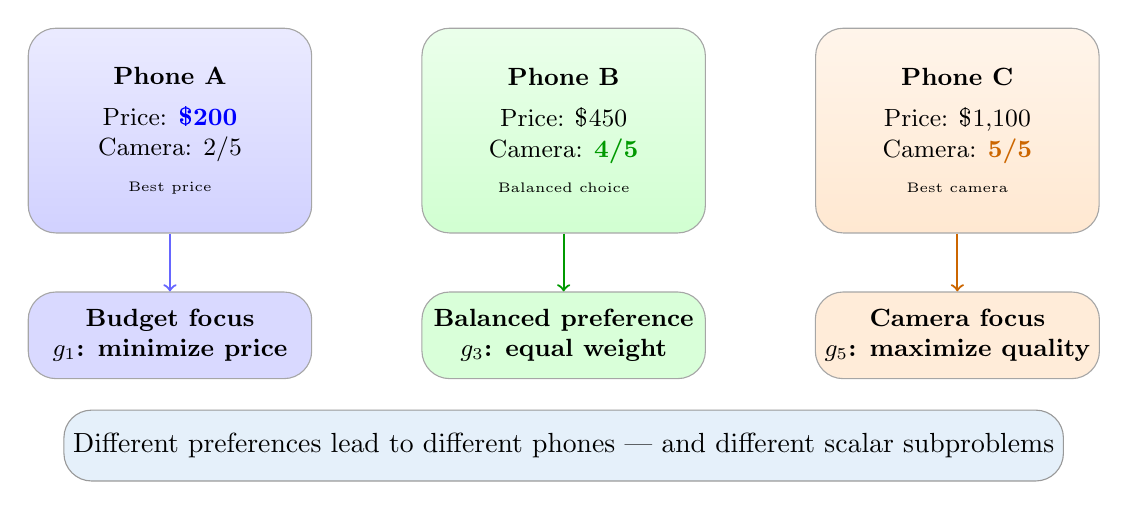
\begin{tikzpicture}[
  phone/.style={
    draw=black!35,
    rounded corners=10pt,
    top color=#1!8,
    bottom color=#1!18,
    minimum width=3.6cm,
    minimum height=2.6cm,
    align=center,
    font=\small
  },
  pref/.style={
    draw=black!35,
    rounded corners=10pt,
    fill=#1!15,
    minimum width=3.6cm,
    minimum height=1.1cm,
    align=center,
    font=\small\bfseries
  }
]

% -------- Phones --------
\node[phone=blue]  (pa) at (0, 0.6)
{\textbf{Phone A}\\[0.4em]
Price: \textcolor{blue}{\textbf{\$200}}\\
Camera: 2/5\\[0.2em]
{\tiny Best price}};

\node[phone=green] (pb) at (5, 0.6)
{\textbf{Phone B}\\[0.4em]
Price: \$450\\
Camera: \textcolor{green!60!black}{\textbf{4/5}}\\[0.2em]
{\tiny Balanced choice}};

\node[phone=orange] (pc) at (10, 0.6)
{\textbf{Phone C}\\[0.4em]
Price: \$1,100\\
Camera: \textcolor{orange!80!black}{\textbf{5/5}}\\[0.2em]
{\tiny Best camera}};

% -------- Preferences (NO text width, NO wrap possible) --------
\node[pref=blue]   (la) at (0,  -2.0)
{Budget focus\\$g_1$: minimize price};

\node[pref=green]  (lb) at (5,  -2.0)
{\mbox{Balanced preference}\\$g_3$: equal weight};

\node[pref=orange] (lc) at (10, -2.0)
{Camera focus\\$g_5$: \mbox{maximize quality}};

% -------- Arrows --------
\draw[->, thick, blue!60]   (pa.south) -- (la.north);
\draw[->, thick, green!60!black]  (pb.south) -- (lb.north);
\draw[->, thick, orange!80!black] (pc.south) -- (lc.north);

% -------- Bottom message --------
\node[
draw=black!40,
rounded corners=10pt,
fill=maincolor!10,
minimum width=12cm,
minimum height=0.9cm,
align=center,
font=\normalsize
] at (5, -3.4)
{Different preferences lead to different phones — and different scalar subproblems};

\end{tikzpicture}
\end{center}
\end{frame}


% -----------------------------------------------------------------------
% SLIDE 33 — Introducing the Weight Vector λ
% -----------------------------------------------------------------------
\begin{frame}{Introducing the Weight Vector $\lambda$}
\begin{center}
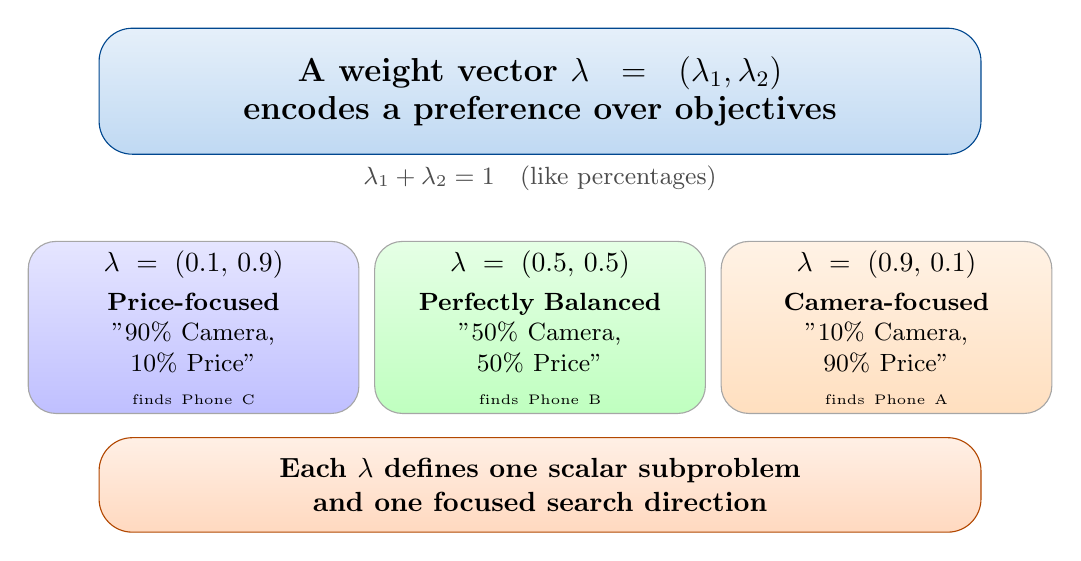
\begin{tikzpicture}[
  ex/.style={
    draw=black!35,
    rounded corners=10pt,
    top color=#1!10,
    bottom color=#1!25,
    minimum width=4.2cm,
    minimum height=1.6cm,
    text width=3.9cm,
    align=center,
    font=\normalsize
  }
]

% -------- Definition card --------
\node[
draw=maincolor!70!black,
rounded corners=12pt,
top color=maincolor!10,
bottom color=maincolor!25,
minimum width=11.2cm,
minimum height=1.6cm,
text width=10.8cm,
align=center,
font=\large\bfseries
] at (0,3.0)
{A weight vector $\lambda = (\lambda_1,\lambda_2)$\\
encodes a preference over objectives};

% -------- Constraint note --------
\node[font=\small, text=black!70] at (0,1.9)
{$\lambda_1 + \lambda_2 = 1 \quad (\text{like percentages})$};

% -------- Examples --------
\node[ex=blue] at (-4.4,0)
{$\lambda = (0.1,\,0.9)$\\[0.3em]
\small \textbf{Price-focused}\\"90\% Camera,\\ 10\% Price"\\
\tiny finds Phone C};

\node[ex=green] at (0,0)
{$\lambda = (0.5,\,0.5)$\\[0.3em]
\small \textbf{Perfectly Balanced}\\"50\% Camera,\\ 50\% Price"\\
\tiny finds Phone B};

\node[ex=orange] at (4.4,0)
{$\lambda = (0.9,\,0.1)$\\[0.3em]
\small \textbf{Camera-focused}\\"10\% Camera,\\ 90\% Price"\\
\tiny finds Phone A};

% -------- Key insight --------
\node[
draw=accentcolor!70!black,
rounded corners=12pt,
top color=accentcolor!10,
bottom color=accentcolor!25,
minimum width=11.2cm,
minimum height=1.2cm,
text width=10.8cm,
align=center,
font=\normalsize\bfseries
] at (0,-2.0)
{Each $\lambda$ defines one scalar subproblem\\
and one focused search direction};

\end{tikzpicture}
\end{center}
\end{frame}


% -----------------------------------------------------------------------
% SLIDE 34 — How Scalarization Works
% -----------------------------------------------------------------------
% \begin{frame}{How Do We Solve Each Sub-Problem? Scalarization}
% \begin{center}
% \begin{tikzpicture}[scale=0.95]

% % -------- Left: Multi-objective --------
% \node[
% draw=red!60!black,
% rounded corners=12pt,
% top color=red!10,
% bottom color=red!25,
% minimum width=4.6cm,
% minimum height=2.5cm,
% text width=4.3cm,
% align=center
% ] (mo) at (-3.6, 0)
% {{\bfseries Multi-objective}\\[0.5em]
% minimize $f_1$ and $f_2$\\[0.4em]
% {\small No single solution\\needs a full front}};

% % -------- Arrow --------
% \draw[->, ultra thick, maincolor!80]
% (-1.1,0) -- (1.1,0)
% node[above, midway, font=\small\bfseries, text=maincolor]
% {scalarize via $\lambda$};

% % -------- Right: Scalar --------
% \node[
% draw=successcolor!60!black,
% rounded corners=12pt,
% top color=successcolor!10,
% bottom color=successcolor!25,
% minimum width=4.6cm,
% minimum height=2.5cm,
% text width=4.3cm,
% align=center
% ] (sc) at (3.6, 0)
% {{\bfseries Scalar subproblem}\\[0.5em]
% minimize $g(\mathbf{f}\mid\lambda)$\\[0.4em]
% {\small One value to optimize\\simple and focused}};

% % -------- Explanation card --------
% \node[
% draw=maincolor!70!black,
% rounded corners=12pt,
% top color=maincolor!10,
% bottom color=maincolor!25,
% text width=10.8cm,
% align=center,
% minimum height=1.1cm,
% font=\normalsize
% ] at (0, -2.2)
% {The weight vector $\lambda$ converts multiple objectives\\into a \textbf{single score} based on a preference};

% % -------- Intuition quote --------
% \node[
% draw=black!40,
% rounded corners=10pt,
% fill=yellow!20,
% text width=10.2cm,
% align=center,
% minimum height=0.9cm,
% font=\small\itshape
% ] at (0, -3.4)
% {``Given my preference $\lambda$, what is the single score of this solution?''};

% \end{tikzpicture}
% \end{center}
% \end{frame}


% -----------------------------------------------------------------------
% SLIDE 35 — Two Classic Scalarization Methods
% -----------------------------------------------------------------------
\begin{frame}{Two Classic Ways to Scalarize}
\begin{center}
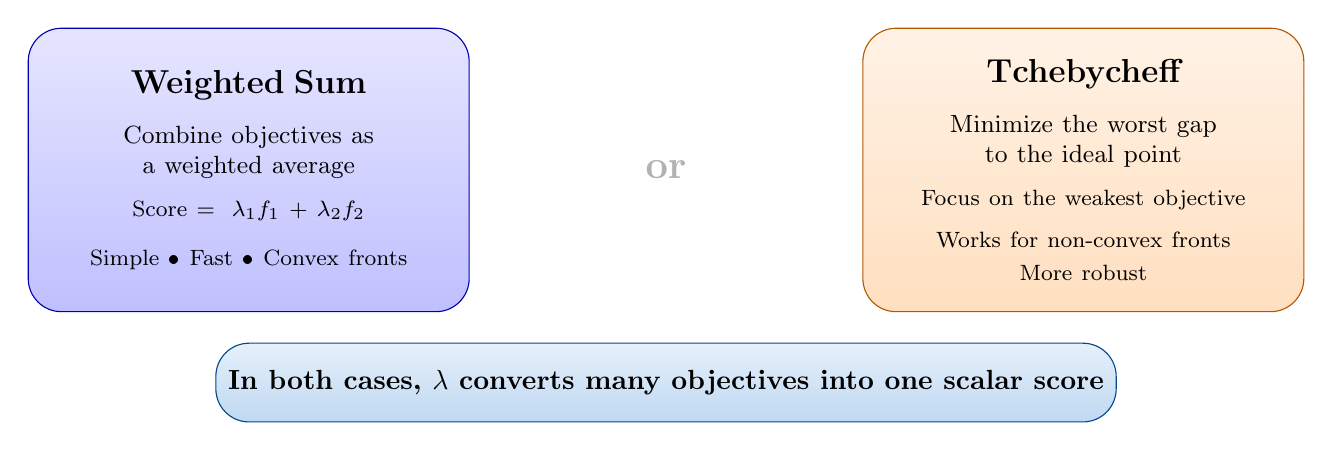
\begin{tikzpicture}[
  method/.style={
    draw=#1!70!black,
    rounded corners=12pt,
    top color=#1!10,
    bottom color=#1!25,
    minimum width=5.6cm,
    minimum height=3.6cm,
    text width=5.2cm,
    align=center
  }
]

% -------- Weighted Sum --------
\node[method=blue] (ws) at (0,0)
{{\bfseries\large Weighted Sum}\\[0.7em]
\small Combine objectives as\\a weighted average\\[0.5em]
{\footnotesize Score $= \lambda_1 f_1 + \lambda_2 f_2$}\\[0.6em]
{\footnotesize Simple \textbullet\ Fast \textbullet\ Convex fronts}};

% -------- OR text --------
\node[font=\Large\bfseries, text=gray!60] at (5.3,0) {or};

% -------- Tchebycheff --------
\node[method=orange] (tc) at (10.6,0)
{{\bfseries\large Tchebycheff}\\[0.7em]
\small Minimize the worst gap\\to the ideal point\\[0.5em]
{\footnotesize Focus on the weakest objective}\\[0.6em]
{\footnotesize Works for non-convex fronts\\More robust}};

% -------- Bottom insight --------
\node[
draw=maincolor!70!black,
rounded corners=12pt,
top color=maincolor!10,
bottom color=maincolor!25,
text width=11.2cm,
align=center,
minimum height=1.0cm,
font=\normalsize\bfseries
] at (5.3,-2.7)
{In both cases, $\lambda$ converts many objectives into one scalar score};

\end{tikzpicture}
\end{center}
\end{frame}


% -----------------------------------------------------------------------
% SLIDE 36 — Geometric View: λ as a Direction in Objective Space
% -----------------------------------------------------------------------
\begin{frame}{$\lambda$ as a Direction: Geometric Intuition}
\begin{center}
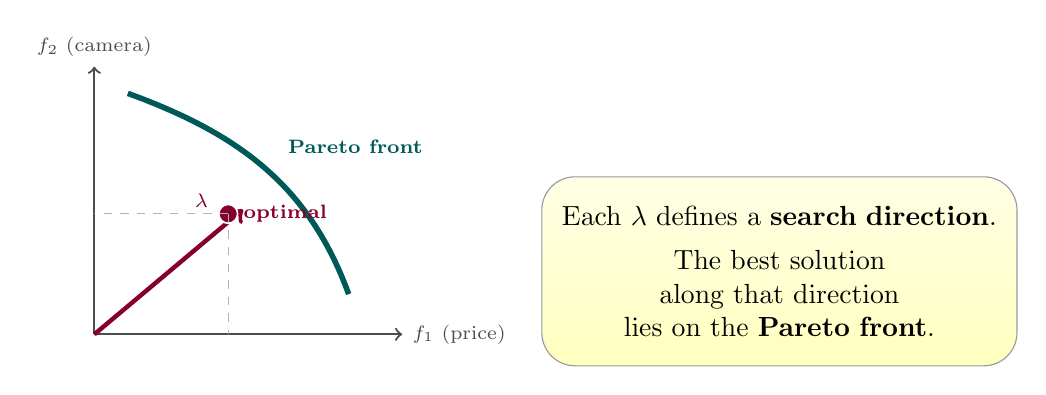
\begin{tikzpicture}

% ================= LEFT: GRAPH =================
\begin{scope}[shift={(-4.2,-0.2)}, scale=0.85]

% Axes
\draw[->, thick, black!70] (0,0) -- (4.6,0)
node[right, font=\scriptsize] {$f_1$ (price)};
\draw[->, thick, black!70] (0,0) -- (0,4.0)
node[above, font=\scriptsize] {$f_2$ (camera)};

% Pareto front (soft teal)
\draw[line width=2pt, teal!70!black]
(0.5,3.6) to[out=-20,in=110] (3.8,0.6);

\node[teal!70!black, font=\scriptsize\bfseries] at (3.9,2.8)
{Pareto front};

% Lambda direction (purple)
\draw[->, ultra thick, purple!70!black] (0,0) -- (40:2.9);

\node[purple!70!black, font=\scriptsize\bfseries] at (1.6,2.0)
{$\lambda$};

% Optimal point (purple highlight)
\filldraw[purple!70!black, draw=white, line width=0.6pt]
(2.0,1.8) circle (4pt);

\node[purple!70!black, font=\scriptsize\bfseries, right=2pt] at (2.0,1.8)
{optimal};

% Projection lines
\draw[dashed, gray!60] (2.0,1.8) -- (2.0,0);
\draw[dashed, gray!60] (2.0,1.8) -- (0,1.8);

\end{scope}

% ================= RIGHT: TEXT BOX =================
\node[
draw=black!40,
rounded corners=12pt,
top color=yellow!10,
bottom color=yellow!25,
text width=5.8cm,
align=center,
minimum height=2.4cm,
font=\normalsize
] at (4.5,0.6)
{Each $\lambda$ defines a \textbf{search direction}.\\[0.4em]
The best solution along that direction\\
lies on the \textbf{Pareto front}.};

\end{tikzpicture}
\end{center}
\end{frame}


% -----------------------------------------------------------------------
% SLIDE 37 — Many λ → Many Points on the Front
% -----------------------------------------------------------------------
\begin{frame}{Many $\lambda$ Directions $\rightarrow$ Many Pareto Points}
\begin{center}
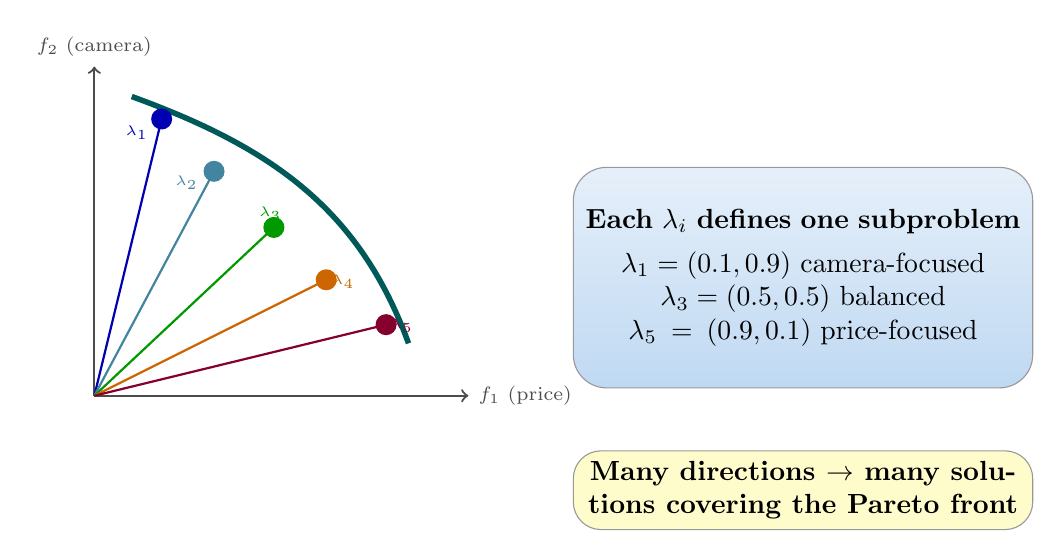
\begin{tikzpicture}

% ================= LEFT: GRAPH =================
\begin{scope}[shift={(-4.2,-0.2)}, scale=0.95]

% Axes
\draw[->, thick, black!70] (0,0) -- (5.0,0)
node[right, font=\scriptsize] {$f_1$ (price)};
\draw[->, thick, black!70] (0,0) -- (0,4.4)
node[above, font=\scriptsize] {$f_2$ (camera)};

% Pareto front (reference curve)
\draw[line width=2pt, teal!70!black]
(0.5,4.0) to[out=-20,in=110] (4.2,0.7);

% --- Lambda arrows that END on PF points ---
\draw[->, thick, blue!70!black]   (0,0) -- (0.9,3.7)
node[pos=0.95, left, font=\tiny] {$\lambda_1$};

\draw[->, thick, cyan!60!black]   (0,0) -- (1.6,3.0)
node[pos=0.95, left, font=\tiny] {$\lambda_2$};

\draw[->, thick, green!60!black]  (0,0) -- (2.4,2.25)
node[pos=0.98, above, font=\tiny] {$\lambda_3$};

\draw[->, thick, orange!80!black] (0,0) -- (3.1,1.55)
node[pos=0.98, right, font=\tiny] {$\lambda_4$};

\draw[->, thick, purple!70!black] (0,0) -- (3.9,0.95)
node[pos=0.98, right, font=\tiny] {$\lambda_5$};

% Points on PF (same coordinates as arrow tips)
\fill[blue!70!black]   (0.9,3.7) circle (4pt);
\fill[cyan!60!black]   (1.6,3.0) circle (4pt);
\fill[green!60!black]  (2.4,2.25) circle (4pt);
\fill[orange!80!black] (3.1,1.55) circle (4pt);
\fill[purple!70!black] (3.9,0.95) circle (4pt);

\end{scope}

% ================= RIGHT: INFO BOX 1 (HARD RIGHT) =================
\node[
draw=black!40,
rounded corners=12pt,
top color=maincolor!10,
bottom color=maincolor!25,
text width=5.6cm,
align=center,
minimum height=2.8cm,
font=\normalsize
] at (4.8,1.3)
{\centering
\textbf{Each $\lambda_i$ defines one subproblem}\\[0.4em]
$\lambda_1=(0.1,0.9)$ camera-focused\\
$\lambda_3=(0.5,0.5)$ balanced\\
$\lambda_5=(0.9,0.1)$ price-focused};

% ================= RIGHT: INFO BOX 2 (HARD RIGHT) =================
\node[
draw=black!40,
rounded corners=10pt,
fill=yellow!20,
text width=5.6cm,
align=center,
minimum height=1.0cm,
font=\normalsize\bfseries
] at (4.8,-1.4)
{Many directions $\rightarrow$ many solutions covering the Pareto front};

\end{tikzpicture}
\end{center}
\end{frame}


% -----------------------------------------------------------------------
% SLIDE 38 — Each λ Owns One Region
% -----------------------------------------------------------------------
\begin{frame}{Each $\lambda$ ``Owns'' One Region of the Pareto Front}
\begin{center}
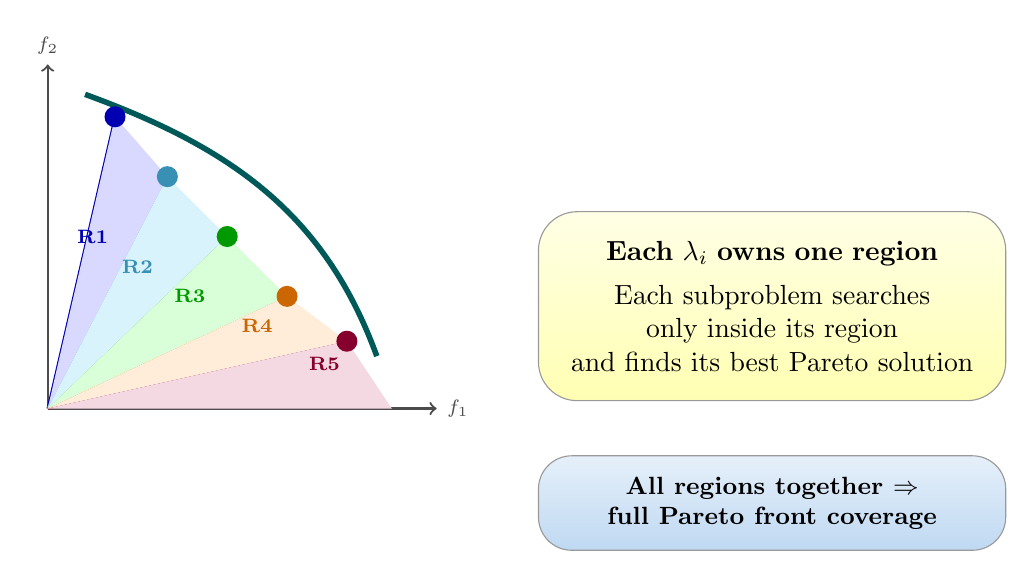
\begin{tikzpicture}

% ================= LEFT: GRAPH =================
\begin{scope}[shift={(-4.3,-0.1)}, scale=0.95]

% Axes
\draw[->, thick, black!70] (0,0) -- (5.2,0) node[right, font=\scriptsize] {$f_1$};
\draw[->, thick, black!70] (0,0) -- (0,4.6) node[above, font=\scriptsize] {$f_2$};

% Pareto front
\draw[line width=2pt, teal!70!black]
(0.5,4.2) to[out=-20,in=110] (4.4,0.7);

% --- PF points (arrow tips) ---
\coordinate (p1) at (0.9,3.9);
\coordinate (p2) at (1.6,3.1);
\coordinate (p3) at (2.4,2.3);
\coordinate (p4) at (3.2,1.5);
\coordinate (p5) at (4.0,0.9);

% --- Lambda arrows ---
\draw[->, thick, blue!70!black]   (0,0) -- (p1);
\draw[->, thick, cyan!70!black]   (0,0) -- (p2);
\draw[->, thick, green!60!black]  (0,0) -- (p3);
\draw[->, thick, orange!80!black] (0,0) -- (p4);
\draw[->, thick, purple!70!black] (0,0) -- (p5);

% --- Region wedges ---
\fill[blue!15]   (0,0) -- (p1) -- (p2) -- cycle;
\fill[cyan!15]   (0,0) -- (p2) -- (p3) -- cycle;
\fill[green!15]  (0,0) -- (p3) -- (p4) -- cycle;
\fill[orange!15] (0,0) -- (p4) -- (p5) -- cycle;
\fill[purple!15] (0,0) -- (p5) -- (4.6,0) -- cycle;

% --- PF points ---
\fill[blue!70!black]   (p1) circle (4pt);
\fill[cyan!70!black]   (p2) circle (4pt);
\fill[green!60!black]  (p3) circle (4pt);
\fill[orange!80!black] (p4) circle (4pt);
\fill[purple!70!black] (p5) circle (4pt);

% --- Region labels ---
\node[blue!70!black,   font=\scriptsize\bfseries] at (0.6,2.3) {R1};
\node[cyan!70!black,   font=\scriptsize\bfseries] at (1.2,1.9) {R2};
\node[green!60!black,  font=\scriptsize\bfseries] at (1.9,1.5) {R3};
\node[orange!80!black, font=\scriptsize\bfseries] at (2.8,1.1) {R4};
\node[purple!70!black, font=\scriptsize\bfseries] at (3.7,0.6) {R5};

\end{scope}

% ================= RIGHT: BOX 1 =================
\node[
draw=black!40,
rounded corners=14pt,
top color=yellow!10,
bottom color=yellow!30,
text width=5.7cm,
align=center,
minimum height=2.4cm,
font=\normalsize
] at (4.9,1.2)
{\textbf{Each $\lambda_i$ owns one region}\\[0.4em]
Each subproblem searches only inside its region\\
and finds its best Pareto solution};

% ================= RIGHT: BOX 2 =================
\node[
draw=black!40,
rounded corners=12pt,
top color=maincolor!10,
bottom color=maincolor!25,
text width=5.7cm,
align=center,
minimum height=1.2cm,
font=\small\bfseries
] at (4.9,-1.3)
{All regions together $\Rightarrow$ full Pareto front coverage};

\end{tikzpicture}
\end{center}
\end{frame}


% -----------------------------------------------------------------------
% SLIDE 39 — Few Weight Vectors → Sparse Coverage
% -----------------------------------------------------------------------
\begin{frame}{Few Weight Vectors $\rightarrow$ Sparse Coverage}
\begin{center}
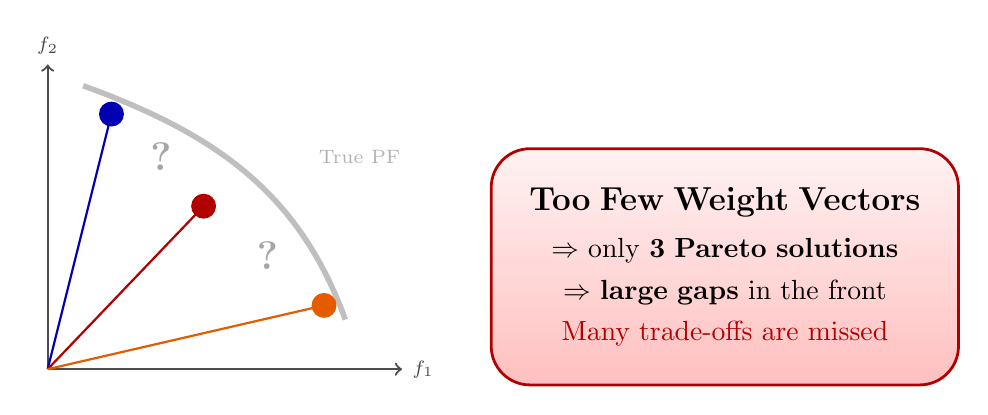
\begin{tikzpicture}

% ================= LEFT: GRAPH =================
\begin{scope}[shift={(-4.0,-0.1)}, scale=0.9]

% Axes
\draw[->, thick, black!70] (0,0) -- (5.0,0) node[right, font=\scriptsize] {$f_1$};
\draw[->, thick, black!70] (0,0) -- (0,4.3) node[above, font=\scriptsize] {$f_2$};

% True Pareto front
\draw[line width=2pt, gray!50]
(0.5,4.0) to[out=-20,in=110] (4.2,0.7);
\node[gray!60, font=\scriptsize] at (4.4,3.0) {True PF};

% PF points
\coordinate (p1) at (0.9,3.6);
\coordinate (p2) at (2.2,2.3);
\coordinate (p3) at (3.9,0.9);

% Arrows
\draw[->, thick, blue!70!black]    (0,0) -- (p1);
\draw[->, thick, red!70!black]     (0,0) -- (p2);
\draw[->, thick, accentcolor!90!black] (0,0) -- (p3);

% Found solutions
\fill[blue!70!black]    (p1) circle (5pt);
\fill[red!70!black]     (p2) circle (5pt);
\fill[accentcolor!90!black] (p3) circle (5pt);

% Missing regions
\node[gray!70, font=\Large\bfseries] at (1.6,3.0) {?};
\node[gray!70, font=\Large\bfseries] at (3.1,1.6) {?};

\end{scope}

% ================= RIGHT: VIBRANT BOX =================
\node[
draw=red!70!black,
line width=1pt,
rounded corners=14pt,
top color=red!5,
bottom color=red!25,
text width=5.7cm,
align=center,
minimum height=3.0cm,
font=\normalsize
] at (4.6,1.2)
{\textbf{\large Too Few Weight Vectors}\\[0.5em]
$\Rightarrow$ only \textbf{3 Pareto solutions}\\[0.3em]
$\Rightarrow$ \textbf{large gaps} in the front\\[0.3em]
\textcolor{red!70!black}{Many trade-offs are missed}};

\end{tikzpicture}
\end{center}
\end{frame}


% -----------------------------------------------------------------------
% SLIDE 40 — Many Weight Vectors → Uniform Coverage
% -----------------------------------------------------------------------
\begin{frame}{Many Weight Vectors $\rightarrow$ Uniform Coverage}
\begin{center}
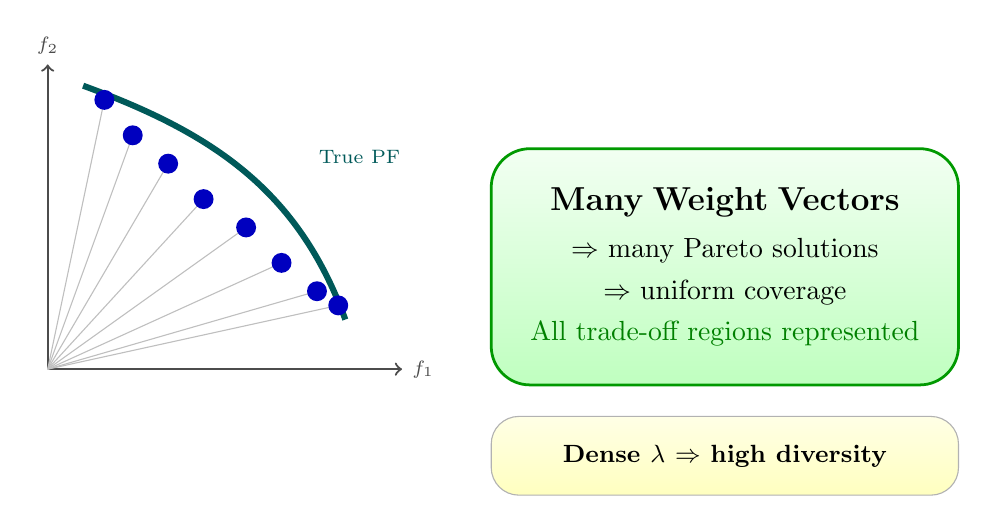
\begin{tikzpicture}

% ================= LEFT: GRAPH =================
\begin{scope}[shift={(-4.0,-0.1)}, scale=0.9]

% Axes
\draw[->, thick, black!70] (0,0) -- (5.0,0) node[right, font=\scriptsize] {$f_1$};
\draw[->, thick, black!70] (0,0) -- (0,4.3) node[above, font=\scriptsize] {$f_2$};

% True Pareto front
\draw[line width=2.2pt, teal!70!black]
(0.5,4.0) to[out=-20,in=110] (4.2,0.7);
\node[teal!70!black, font=\scriptsize] at (4.4,3.0) {True PF};

% PF points (aligned)
\coordinate (p1) at (0.8,3.8);
\coordinate (p2) at (1.2,3.3);
\coordinate (p3) at (1.7,2.9);
\coordinate (p4) at (2.2,2.4);
\coordinate (p5) at (2.8,2.0);
\coordinate (p6) at (3.3,1.5);
\coordinate (p7) at (3.8,1.1);
\coordinate (p8) at (4.1,0.9);

% Lambda arrows
\foreach \p in {p1,p2,p3,p4,p5,p6,p7,p8}
  \draw[->, thin, gray!50] (0,0) -- (\p);

% Found solutions
\foreach \p in {p1,p2,p3,p4,p5,p6,p7,p8}
  \fill[blue!75!black] (\p) circle (4pt);

\end{scope}

% ================= RIGHT: SUCCESS BOX =================
\node[
draw=green!60!black,
line width=1pt,
rounded corners=14pt,
top color=green!5,
bottom color=green!25,
text width=5.7cm,
align=center,
minimum height=3.0cm,
font=\normalsize
] at (4.6,1.2)
{\textbf{\large Many Weight Vectors}\\[0.5em]
$\Rightarrow$ many Pareto solutions\\[0.3em]
$\Rightarrow$ uniform coverage\\[0.3em]
\textcolor{green!50!black}{All trade-off regions represented}};

% Emphasis strip
\node[
draw=black!30,
rounded corners=10pt,
top color=yellow!10,
bottom color=yellow!25,
text width=5.7cm,
align=center,
minimum height=1.0cm,
font=\small\bfseries
] at (4.6,-1.2)
{Dense $\lambda$ $\Rightarrow$ high diversity};

\end{tikzpicture}
\end{center}
\end{frame}


% -----------------------------------------------------------------------
% SLIDE 41 — Why Decomposition Is Powerful: Local Focus
% -----------------------------------------------------------------------
\begin{frame}{Why Is Decomposition So Powerful? \#1: Local Focus}
\begin{center}
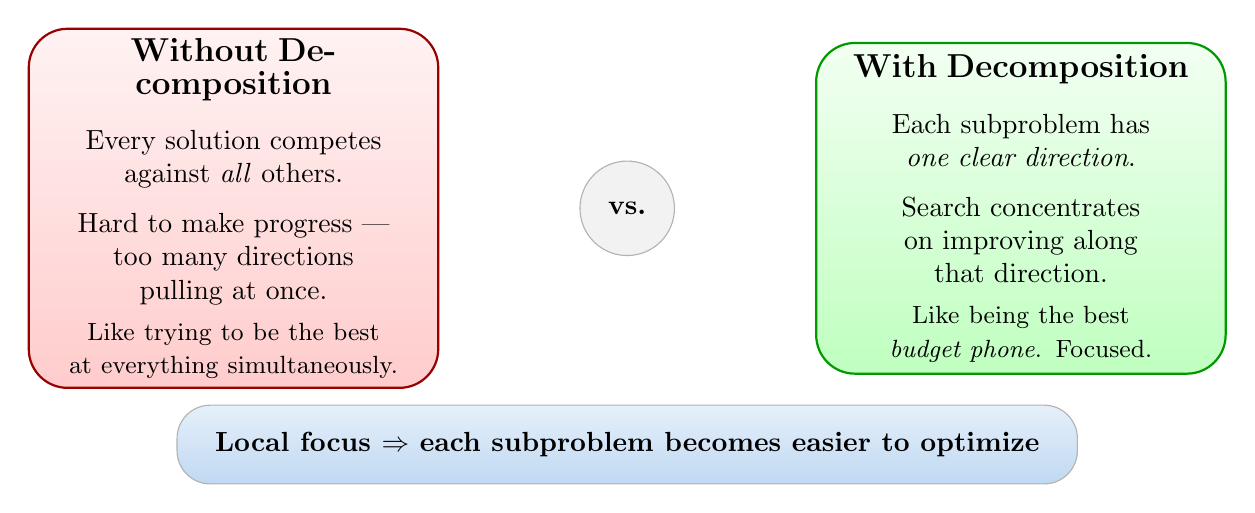
\begin{tikzpicture}

% ================= LEFT: WITHOUT DECOMPOSITION =================
\node[
draw=red!60!black,
line width=0.8pt,
rounded corners=14pt,
top color=red!5,
bottom color=red!20,
minimum width=5.2cm,
minimum height=4.2cm,
text width=4.9cm,
align=center,
font=\normalsize
] (chaos) at (0, 0)
{\textbf{\large Without Decomposition}\\[0.8em]
Every solution competes\\
against \textit{all} others.\\[0.6em]
Hard to make progress —\\
too many directions\\
pulling at once.\\[0.4em]
{\small Like trying to be the best\\
at everything simultaneously.}};

% ================= VS BADGE =================
\node[
draw=black!30,
circle,
fill=gray!10,
minimum size=1.2cm,
font=\bfseries
] at (5.0,0) {vs.};

% ================= RIGHT: WITH DECOMPOSITION =================
\node[
draw=green!60!black,
line width=0.8pt,
rounded corners=14pt,
top color=green!5,
bottom color=green!25,
minimum width=5.2cm,
minimum height=4.2cm,
text width=4.9cm,
align=center,
font=\normalsize
] (focus) at (10.0, 0)
{\textbf{\large With Decomposition}\\[0.8em]
Each subproblem has\\
\textit{one clear direction}.\\[0.6em]
Search concentrates\\
on improving along\\
that direction.\\[0.4em]
{\small Like being the best\\
\textit{budget phone}. Focused.}};

% ================= BOTTOM TAKEAWAY STRIP =================
\node[
draw=black!30,
rounded corners=12pt,
top color=maincolor!10,
bottom color=maincolor!25,
text width=11.2cm,
align=center,
minimum height=1.0cm,
font=\normalsize\bfseries
] at (5.0, -3.0)
{Local focus $\Rightarrow$ each subproblem becomes easier to optimize};

\end{tikzpicture}
\end{center}
\end{frame}


% -----------------------------------------------------------------------
% SLIDE 42 — Why Decomposition Is Powerful: Natural Diversity
% -----------------------------------------------------------------------
\begin{frame}{Why Is Decomposition So Powerful? \#2: Natural Diversity}
\begin{center}
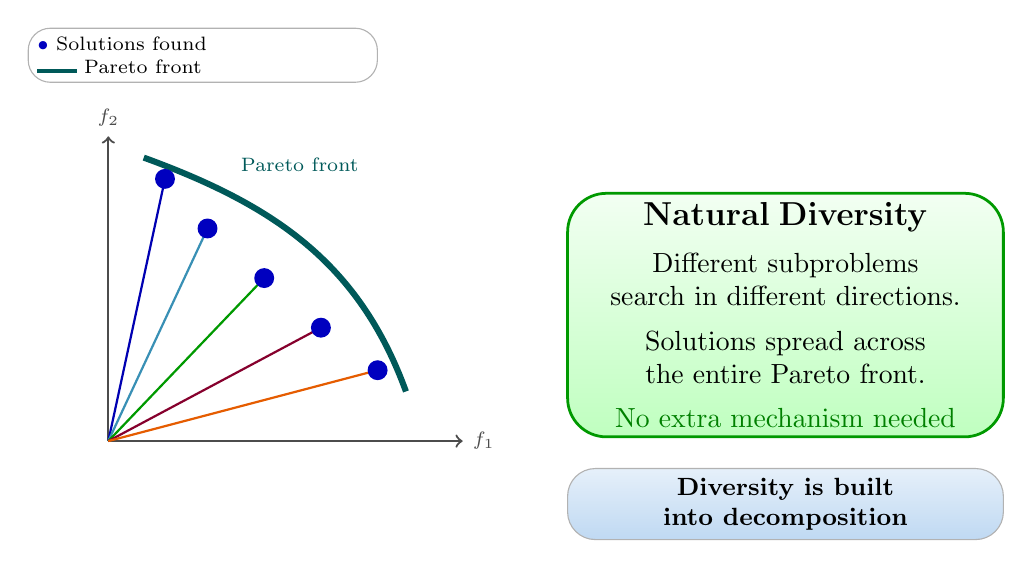
\begin{tikzpicture}

% ================= LEFT: GRAPH =================
\begin{scope}[shift={(-4.0,-0.1)}, scale=0.9]

% Axes
\draw[->, thick, black!70] (0,0) -- (5.0,0)
node[right, font=\scriptsize] {$f_1$};
\draw[->, thick, black!70] (0,0) -- (0,4.3)
node[above, font=\scriptsize] {$f_2$};

% Pareto front
\draw[line width=2.2pt, teal!70!black]
(0.5,4.0) to[out=-20,in=110] (4.2,0.7);

% PF label (lowered slightly)
\node[teal!70!black, font=\scriptsize] at (2.7,3.9) {Pareto front};

% PF points
\coordinate (p1) at (0.8,3.7);
\coordinate (p2) at (1.4,3.0);
\coordinate (p3) at (2.2,2.3);
\coordinate (p4) at (3.0,1.6);
\coordinate (p5) at (3.8,1.0);

% Lambda arrows
\draw[->, thick, blue!70!black]   (0,0) -- (p1);
\draw[->, thick, cyan!70!black]   (0,0) -- (p2);
\draw[->, thick, green!60!black]  (0,0) -- (p3);
\draw[->, thick, purple!70!black] (0,0) -- (p4);
\draw[->, thick, accentcolor!90!black] (0,0) -- (p5);

% Solutions on PF
\foreach \p in {p1,p2,p3,p4,p5}
  \fill[blue!75!black] (\p) circle (4pt);

\end{scope}

% ================= LEGEND ABOVE GRAPH (RAISED) =================
\node[
draw=black!30,
rounded corners=8pt,
fill=white,
text width=4.2cm,
align=left,
font=\scriptsize
] at (-2.8,4.8)
{\textcolor{blue!75!black}{$\bullet$} Solutions found\\
\textcolor{teal!70!black}{\rule{0.5cm}{1.5pt}} Pareto front};

% ================= RIGHT: MAIN BOX =================
\node[
draw=green!60!black,
line width=1pt,
rounded corners=14pt,
top color=green!5,
bottom color=green!25,
text width=5.3cm,
align=center,
minimum height=2.8cm,
font=\normalsize
] at (4.6,1.5)
{\textbf{\large Natural Diversity}\\[0.5em]
Different subproblems\\
search in different directions.\\[0.4em]
Solutions spread across\\
the entire Pareto front.\\[0.4em]
\textcolor{green!50!black}{No extra mechanism needed}};

% ================= TAKEAWAY STRIP =================
\node[
draw=black!30,
rounded corners=10pt,
top color=maincolor!10,
bottom color=maincolor!25,
text width=5.3cm,
align=center,
minimum height=0.9cm,
font=\small\bfseries
] at (4.6,-0.9)
{Diversity is built into decomposition};

\end{tikzpicture}
\end{center}
\end{frame}


% -----------------------------------------------------------------------
% SLIDE 43 — Why Decomposition Is Powerful: No Global Ranking
% -----------------------------------------------------------------------
\begin{frame}{Why Is Decomposition So Powerful? \#3: No Global Ranking Needed}
\begin{center}
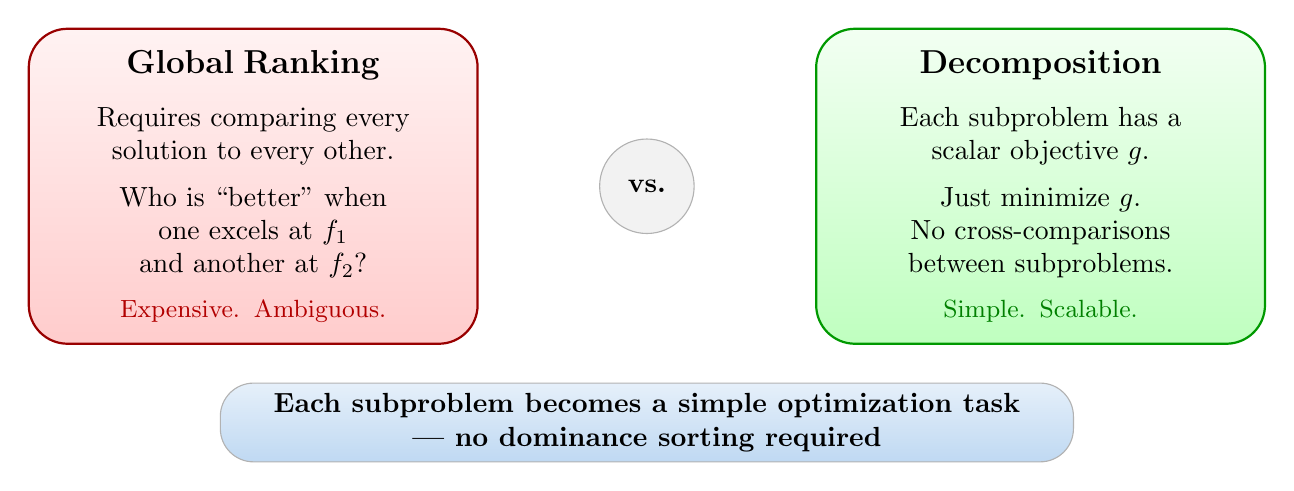
\begin{tikzpicture}

% ================= LEFT: GLOBAL RANKING =================
\node[
draw=red!60!black,
line width=0.8pt,
rounded corners=14pt,
top color=red!5,
bottom color=red!20,
minimum width=5.7cm,
minimum height=4.0cm,
text width=5.4cm,
align=center,
font=\normalsize
] at (0, 0.4)
{\textbf{\large Global Ranking}\\[0.7em]
Requires comparing every\\
solution to every other.\\[0.5em]
Who is ``better'' when\\
one excels at $f_1$\\
and another at $f_2$?\\[0.4em]
{\small \textcolor{red!70!black}{Expensive. Ambiguous.}}};

% ================= VS BADGE =================
\node[
draw=black!30,
circle,
fill=gray!10,
minimum size=1.2cm,
font=\bfseries
] at (5.0,0.4) {vs.};

% ================= RIGHT: DECOMPOSITION =================
\node[
draw=green!60!black,
line width=0.8pt,
rounded corners=14pt,
top color=green!5,
bottom color=green!25,
minimum width=5.7cm,
minimum height=4.0cm,
text width=5.4cm,
align=center,
font=\normalsize
] at (10.0, 0.4)
{\textbf{\large Decomposition}\\[0.7em]
Each subproblem has a\\
scalar objective $g$.\\[0.5em]
Just minimize $g$.\\
No cross-comparisons\\
between subproblems.\\[0.4em]
{\small \textcolor{green!50!black}{Simple. Scalable.}}};

% ================= BOTTOM TAKEAWAY STRIP =================
\node[
draw=black!30,
rounded corners=12pt,
top color=maincolor!10,
bottom color=maincolor!25,
text width=10.6cm,
align=center,
minimum height=1.0cm,
font=\normalsize\bfseries
] at (5.0, -2.6)
{Each subproblem becomes a simple optimization task\\
— no dominance sorting required};

\end{tikzpicture}
\end{center}
\end{frame}


% -----------------------------------------------------------------------
% SLIDE 44 — The Foundation: Decomposition
% -----------------------------------------------------------------------
\begin{frame}{}
\begin{center}

\vspace{1.0em}
{\large\itshape All of this — directions, subproblems, scalarization, coverage — leads to one conclusion:}

\vspace{1.8em}


\begin{tikzpicture}

% Glow layer
\node[
draw=maincolor!30,
line width=2pt,
rounded corners=22pt,
fill=maincolor!5,
minimum width=12.6cm,
minimum height=3.4cm
] at (0,0) {};

% Main vibrant box
\node[
draw=maincolor!80!black,
line width=1.5pt,
rounded corners=20pt,
top color=maincolor!20,
bottom color=maincolor!35,
minimum width=12.2cm,
minimum height=3.1cm,
text width=11.8cm,
align=center
] at (0,0)
{{\Huge\bfseries\color{maincolor} Decomposition}\\[0.6em]
{\LARGE\bfseries is the foundation of}\\[0.3em]
{\LARGE\bfseries\color{accentcolor}MOEA/D}};

\end{tikzpicture}

\vspace{1.6em}


\begin{tikzpicture}
\node[
draw=accentcolor!60!black,
line width=1pt,
rounded corners=12pt,
top color=accentcolor!10,
bottom color=accentcolor!25,
text width=10.8cm,
align=center,
minimum height=1.1cm,
font=\normalsize\bfseries
]
{Every design decision in MOEA/D follows from this one idea};
\end{tikzpicture}

\end{center}
\end{frame}


% -----------------------------------------------------------------------
% SLIDE 45 — Handover to Speaker 3
% -----------------------------------------------------------------------
\begin{frame}{So Far: Subproblems. Next: Making Them Cooperate.}
\begin{center}
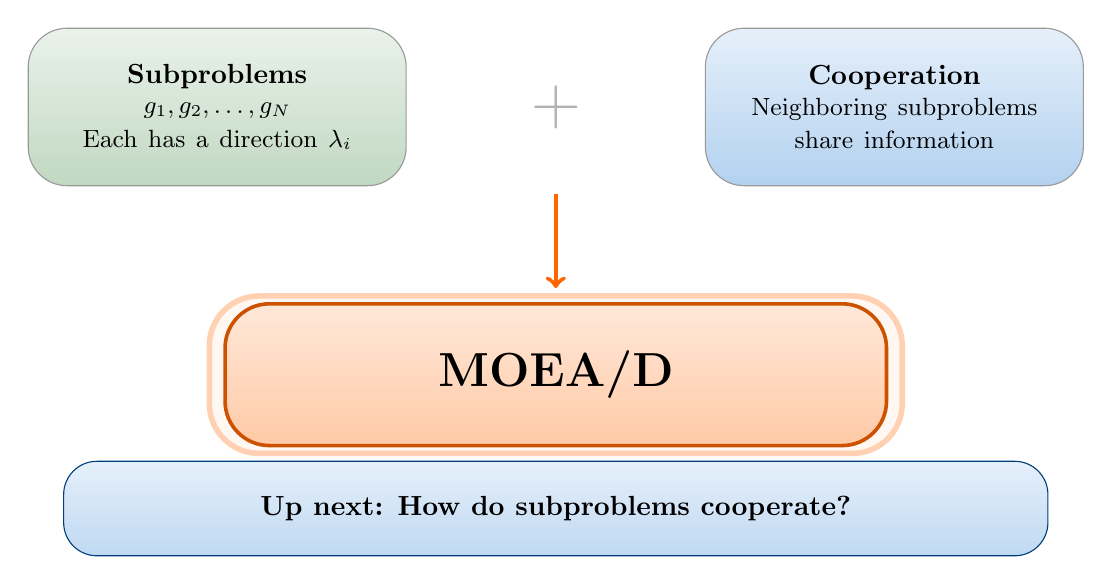
\begin{tikzpicture}[
  box/.style={
    draw=black!40,
    rounded corners=14pt,
    top color=#1!10,
    bottom color=#1!30,
    minimum width=4.8cm,
    minimum height=2.0cm,
    text width=4.5cm,
    align=center,
    font=\normalsize\bfseries
  }
]

% Left: Subproblems
\node[box=successcolor] (sub) at (0, 1.8)
{Subproblems\\
{\small\normalfont $g_1, g_2, \ldots, g_N$\\
Each has a direction $\lambda_i$}};

% Plus sign
\node[font=\Huge\bfseries, text=gray!60] at (4.3, 1.8) {$+$};

% Right: Cooperation
\node[box=maincolor] (coop) at (8.6, 1.8)
{Cooperation\\
{\small\normalfont Neighboring subproblems\\
share information}};

% Arrow down to MOEA/D
\draw[->, ultra thick, accentcolor] (4.3, 0.7) -- (4.3, -0.5);

% Glow layer
\node[
draw=accentcolor!30,
line width=2pt,
rounded corners=18pt,
fill=accentcolor!5,
minimum width=8.8cm,
minimum height=2.0cm
] at (4.3, -1.6) {};

% MOEA/D box
\node[
draw=accentcolor!80!black,
line width=1.3pt,
rounded corners=16pt,
top color=accentcolor!15,
bottom color=accentcolor!35,
minimum width=8.4cm,
minimum height=1.8cm,
text width=8.0cm,
align=center,
font=\LARGE\bfseries
] at (4.3, -1.6)
{MOEA/D};

% Bottom strip — NO WORD BREAK
\node[
draw=maincolor!60!black,
rounded corners=12pt,
top color=maincolor!10,
bottom color=maincolor!25,
minimum width=12.5cm,
minimum height=1.2cm,
align=center,
font=\normalsize\bfseries
] at (4.3, -3.3)
{Up next: How do subproblems cooperate?};

\end{tikzpicture}
\end{center}
\end{frame}

\end{document}